\documentclass[./main.tex]{subfiles}
\begin{document}


%desarrollo embrionario
El desarrollo embrionario de un mamífero comienza con el cigoto, una sola célula que tiene origen en la fecundación entre el oocito y el espermatozoide. A partir del cigoto se desarrolla el embrión, que durante el desarrollo embrionario dará origen a muchos tipos de células dispuestas en un patrón final de gran complejidad y precisión, el organismo maduro (figura \ref{C1_fig:mouse_emb_dev}) \cite{Alberts2008}. 


 \begin{figure}
    \centering
    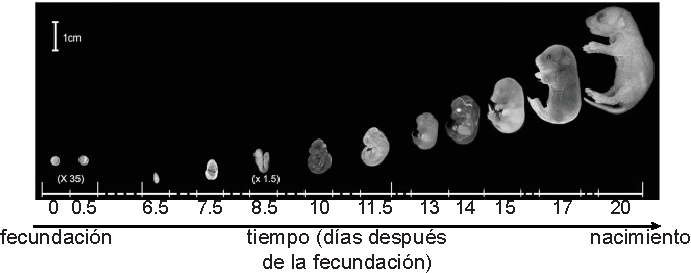
\includegraphics[width=1\columnwidth]{figures/chapter1/C1_mouse_emb_dev.pdf}
    \caption{\textbf{El desarrollo embrionario da origen al organismo maduro a partir de una sola célula.} Estadíos del desarrollo embrionario del ratón, desde la fecundación hasta el nacimiento, que sucede aproximadamente 20 días después de la concepción. La escala temporal no es lineal y está indicada en términos de días después de la fecundación. Figura adaptada de \cite{Xue2013}.}
    \label{C1_fig:mouse_emb_dev}
\end{figure}


%tipos celulares
Los tipos celulares del organismo maduro difieren drásticamente tanto en su estructura como en su función, y cada uno cumple tareas específicas. Como ilustración, las neuronas son las encargadas de transportar los impulsos nerviosos, o las células hepáticas participan en muchos procesos metabólicos como en la digestión y la desintoxicación del alcohol y otras drogas  (figura \ref{C1_fig:cell_types}). Por ejemplo, el ratón adulto tiene más de 120 tipos celulares y, aunque todos ellos comparten el mismo material genético, cada tipo celular expresa diferentes conjuntos de ARN y proteínas que le confieren distintas morfología y funcionalidad \cite{Zhang2021,Weinberger2016,Schrode2013}.


 \begin{figure}
    \centering
    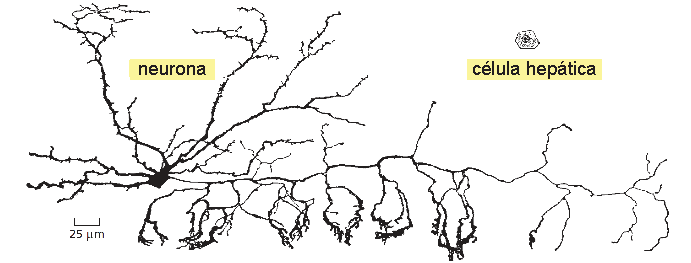
\includegraphics[width=1\columnwidth]{figures/chapter1/C1_cell_types.pdf}
    \caption{\textbf{Los tipos celulares del organismo maduro difieren drásticamente tanto en su estructura como en su función.} Representación de una neurona de la retina (izquierda) y una célula hepática (derecha) dibujadas en la misma escala. Estas dos células de forma, tamaño, y funciones distintas tienen el mismo material genético, pero expresan diferentes conjuntos de ARN y proteínas. Figura adaptada de \cite{Alberts2008}.}
    \label{C1_fig:cell_types}
\end{figure}

%diferenciación celular
Para dar lugar a la diversidad celular presente en el organismo maduro, durante el desarrollo embrionario las células atraviesan complejos programas de diferenciación celular. En cada evento de diferenciación, se activan e inactivan diversos programas de regulación genética, lo que le confiere a la célula funciones cada vez más específicas. El objetivo general de esta tesis es comprender cómo se activan estos distintos patrones de regulación genética en la diferenciación celular durante el desarrollo embrionario. 


Durante el desarrollo embrionario, para tomar decisiones de destino celular, como dividirse o diferenciarse, las células detectan señales de su entorno, y la procesan junto con información sobre su propio estado interno (figura \ref{C1_fig:signalling}A). Este procedimiento da como resultado una señal intracelular que regula la expresión génica y promueve las decisiones de destino celular. La respuesta de las células a una dada señal suele depender de otras señales que reciben simultáneamente y de su propio estado interno. Entonces, ¿cómo la célula recibe e integra toda esta información, y la resume en la señal intracelular que promueve decisiones de destino celular?

 \begin{figure}
    \centering
    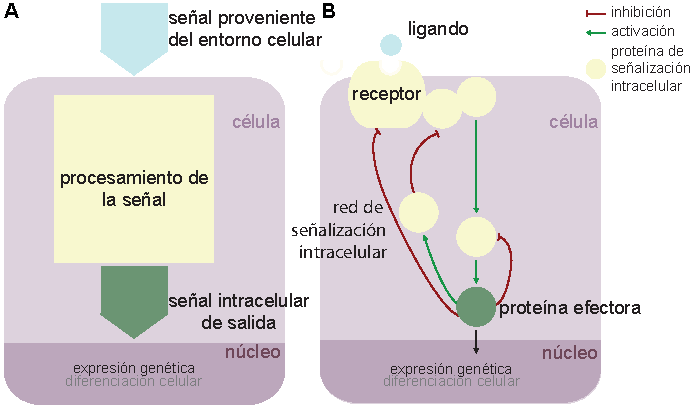
\includegraphics[width=1\columnwidth]{figures/chapter1/C1_signalling.pdf} 
    \caption{\textbf{Las células procesan señales extracelulares junto con información sobre su propio estado interno para tomar decisiones de destino celular.} (A)  Esquema de cómo fluye la información en una célula que recibe una señal extracelular, cuyo procesamiento puede conducir a decisiones de destino celular. (B) Esquema de un sistema de señalización celular, en donde se indica cada uno de sus componentes, incluyendo la red de transducción de señales organizada en conjuntos de motivos de retroalimentación.}
    \label{C1_fig:signalling}
\end{figure}

Este tipo de señales puede provenir de células que emiten la señal, y secretan proteínas o ligandos de señalización extracelular hacia su entorno. La recepción de estas señales por parte de las células que incorporan la señal depende de proteínas receptoras -o receptores- de gran especificidad, que reconocen y se unen al ligando. Los receptores normalmente están localizados en la superficie de la célula que recibe la señal (figura \ref{C1_fig:signalling}B). La unión entre el ligando y el receptor de membrana activa esta proteína receptora, por ejemplo promoviendo su fosforilación. Esta activación desencadena la activación de una o más redes de transducción de señales, redes de proteínas de señalización intracelular normalmente organizadas en conjuntos de motivos de retroalimentación (figura \ref{C1_fig:signalling}B) \cite{Alon2006,Shen2002,Milo2002,Tyson2003,Tyson2010,Alon2007}. Qué motivos de retroalimentación forman la red, y cómo es su disposición depende de la arquitectura específica de cada tipo celular y del procesamiento simultáneo de otras señales intra y extracelulares. Por este motivo, las redes de transducción de señales son las herramientas que la célula dispone para procesar la señal extracelular que recibió, e integrarla con otras señales y su propio estado interno. El procesamiento de señales que surge de estas redes organizadas en conjuntos de motivos de retroalimentación puede convertir una señal simple de ligando en una respuesta dinámica compleja de la proteína que se encuentra al final de la red, comúnmente denominada proteína efectora  (figura \ref{C1_fig:signalling}B) \cite{Antebi2017,Santos2007}. Por ejemplo, en muchos sistemas un aumento gradual de una señal extracelular se convierte en una respuesta abrupta, tipo interruptor, de la proteína efectora. En otros casos, una señal de entrada constante se convierte en una respuesta oscilatoria. 


Los patrones dinámicos de actividad de las proteínas efectoras normalmente resumen la información que surge del procesamiento de señales. Estas proteínas pueden ser reguladoras de la transcripción (figura \ref{C1_fig:signalling}B). Entonces, la posibilidad de que sus patrones dinámicos sean flexibles sugiere que los genes sirven como depósitos de información de control dinámico sobre la combinación de ARN y proteínas que definen un estado fenotípico estable de la célula \cite{Koseska2017}.


En este marco, algunas preguntas que motivan este trabajo son (i) cómo es la forma de la respuesta dinámica de las proteínas efectoras ante distintas señales extracelulares involucradas en la diferenciación celular al principio del desarrollo embrionario, (ii) qué propiedades de esta respuesta dinámica constituyen información sobre los estímulos extracelulares y el estado interno de la célula receptora, (iii) qué características de esta señal miden las células para eventualmente tomar decisiones de destino celular, y (iv) qué tan homogénea es la respuesta de una población de células a una dada señal y en distintos contextos. 


Utilizaremos células madre embrionarias de ratón como organismo modelo para explorar estos interrogantes. Éstas son células derivadas de tejidos del desarrollo embrionario temprano, y son un organismo modelo popular para estudiar diferenciación celular en este contexto biológico. Nos enfocaremos en uno de los sistemas de transducción de señales más importantes durante el desarrollo embrionario temprano y en las células madre embrionarias, que transmite señales de la proteína extracelular FGF4 a través de la red de señalización intracelular RAS/RAF/MEK/ERK, donde ERK es la proteína efectora \cite{Brewer2016}. Si bien la función de esta red es conocida, la dinámica de señalización de ERK es prácticamente desconocida en este contexto del desarrollo. 


%Comprender los mecanismos que gobiernan los procesos de diferenciación celular es crucial para desarrollar técnicas de diferenciación celular dirigida, técnicas sumamente útiles en el desarrollo de la medicina regenerativa, en la investigación de enfermedades o en el monitoreo y testeo de drogas experimentales \cite{Keller2005,Inoue2014}. Como complemento, estos son conocimientos relevantes para desarrollar nuevas tratamientos en los casos en que falla la elección del destino celular, como es el de las enfermedades congénitas y el cáncer.


Para contextualizar, a continuación resumiremos las principales ideas y conocimientos de biología celular y del desarrollo en las que se enmarca el resto del trabajo. Primero describiremos las primeras etapas del desarrollo embrionario. Luego, introduciremos el origen, las principales propiedades, las condiciones de cultivo y los protocolos de diferenciación de las células madre embrionarias. Más adelante introduciremos los sistemas de señalización celular, enfocándonos sistema de señalización FGF/ERK en el contexto del desarrollo embrionario. Repasaremos las propiedades conocidas de la red, y cómo es la actividad de ERK en otros contextos biológicos relevantes. Finalmente, presentaremos los objetivos que perseguimos en esta tesis, el esquema de trabajo que adoptaremos para responderlas, y especularemos sobre el posible impacto de nuestros resultados.



\section{Desarrollo embrionario temprano}
\label{C1_sec:desarrollo_embrionario_temprano}

% desarrollo embrionario temprano 
El desarrollo embrionario temprano abarca desde la fecundación hasta los momentos previos de la implantación del embrión en el útero materno. Luego de la fecundación continúa la segmentación, donde el cigoto se divide células más pequeñas llamadas blastómeros. Los blastómeros a los aproximadamente 3 días luego de la fecundación forman la mórula, una masa compacta de aproximadamente 16 células (figura \ref{C1_fig:des_emb_temprano}) \cite{Gilbert2006}. La mórula origina el blastocisto, compuesto por una capa externa de células, llamada trofoblasto, y una capa interna de células, denominada masa celular interna. Las células pertenecientes a alguno de estos dos grupos no contribuyen a las células del otro grupo, lo que constituye el primer evento de diferenciación en el desarrollo embrionario con consecuencias visibles en la morfología y función de las células  \cite{Dyce1987,Fleming1987}. El trofoblasto eventualmente darán origen a la parte embrionaria de la placenta, y las aproximadamente 13 células de la masa celular interna darán lugar al embrión y a parte del tejido extraembrionario.  


\begin{figure}
    \centering
    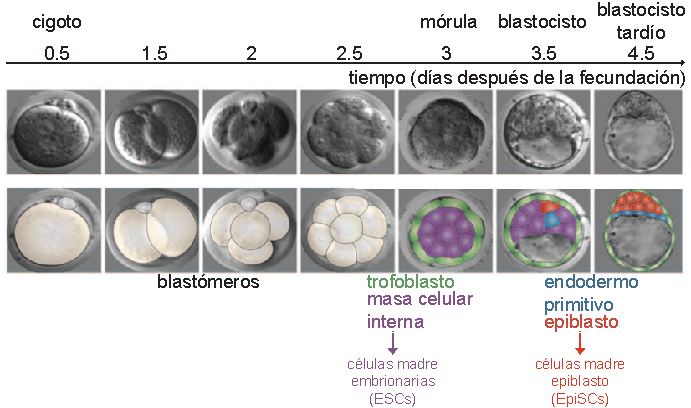
\includegraphics[width=1\columnwidth]{figures/chapter1/C1_des_emb_temprano.pdf} 
    \caption{\textbf{Desarrollo embrionario temprano.} (arriba) Desarrollo del embrión de preimplantación. El tiempo, medido en días después de la fecundación, está indicado en la parte superior de la figura junto con los nombres de los organismos de cada etapa del desarrollo. (abajo) Esquema de los tipos celulares que intervienen en el desarrollo embrionario de preimplantación, codificados en color. Se encuentra también indicado que las células madre embrionarias derivan de la masa celular interna de la mórula, y que las células madre epiblasto provienen del epiblasto del blastocisto. Figura adaptada de \cite{Schrode2013}.}
    \label{C1_fig:des_emb_temprano}
\end{figure}

%durante la cavitación 
A continuación, las células del trofoblasto segregan líquido para crear una cavidad, y la masa celular interna se sitúa en un lado del anillo de células del trofoblasto  (figura \ref{C1_fig:des_emb_temprano}). En adelante, los tejidos tempranos del embrión se generan por la reorganización y diferenciación de las células de la masa celular interna. La primera reorganización ocurre justo antes de la implantación en el útero materno, con la segregación en dos capas: el endodermo primitivo o hipoblasto, y el tejido remanente de la masa celular interna, epiblasto o ectodermo primitivo. Luego de la implantación, las células del endodermo primitivo darán lugar a linajes extraembrionarios que formarán, por ejemplo, el saco vitelino. Por otro lado, las células del epiblasto darán lugar a otra parte del tejido extraembrionario que eventualmente formará por ejemplo el amnios, y al embrión con sus tres capas germinales \cite{Beddington1999,Nakamura2016,Gardner1983}. Es decir, el epiblasto es el tejido del cual derivan todas las células del organismo adulto.


Para este trabajo es relevante cómo se da lugar a la diferenciación de las células de la masa celular interna en células del endodermo primitivo y epiblasto (figura \ref{C1_fig:des_emb_temprano}, entre días $3$ y $4.5$). En el momento previo a la reorganización, las células de la masa celular interna expresan genes marcadores tanto del epiblasto como del endodermo primitivo simultáneamente. Luego, hay una progresión gradual hacia un estado donde estos dos linajes se restringen a un sólo destino celular en un aparente patrón aleatorio comúnmente llamado de sal y pimienta, ya que la expresión de genes específicos de cada linaje se vuelve mutuamente excluyente. Finalmente, los dos tipos celulares se segregan en sus posiciones finales, recubriendo la cavidad del blasticisto tardío \cite{Plusa2008}. 


Es posible modular en experimentos esta decisión sobre el destino de las células para generar un tejido interno del blastocisto completamente compuesto por células del endodermo primitivo o del epiblasto (figura \ref{C1_fig:saltandpepper}A). En el ratón, la diferenciación de las células de la masa interna en el endodermo primitivo depende de la dosis del factor de crecimiento de fibroblastos 4 (FGF4, por \textit{fibroblast grow factor 4}) \cite{Kang2013,Krawchuk2013,Ohnishi2014}. Por un lado, cultivando embriones en FGF4 exógeno es posible generar un tejido interno completamente compuesto por células del endodermo primitivo. Por otro lado, inhibiendo los receptores FGFr -es decir, la recepción de la señal de FGF4 extracelular- se genera uno completamente compuesto por células del epiblasto \cite{Yamanaka2010,Grabarek2012}. Además, la estimulación de los receptores FGFr principalmente activa la vía de transducción de señales compuesta por las quinasas RAS/RAF/MEK/ERK \cite{Brewer2016}. La inhibición de MEK también da lugar a un tejido desprovisto de endodermo primitivo, indicando que la señalización de ERK también se requiere para la formación del endodermo primitivo, y muy probablemente es la responsable de mediar la función de FGFr (figura \ref{C1_fig:saltandpepper}A) \cite{Nichols2009}.  


A partir de estos resultados, se sostiene que la regulación del nivel de la señal FGF/RAS/RAF /MEK/ERK es esencial y suficiente para la segregación de estos dos linajes en el blastocisto, y que el patrón de sal y pimienta aparece de manera estocástica dependiendo de los niveles de señalización de la red. Es decir, cuando se bloquea la señal, las células expresan marcadores de células del epiblasto. En contraposición, a valores altos de señal, expresan marcadores de endodermo primitivo. Se cree que a valores intermedios de señalización -probables en embriones- las células de la masa celular interna responderán a la señal de manera aleatoria (figura \ref{C1_fig:saltandpepper}B). En este modelo, el nivel de la señal controla la proporción de células capaces de responder, y las variaciones intrínsecas y extrínsecas (ruido) en las células individuales determinan si éstas responden a la señal. Además, se observó que este proceso es reversible entre los $3.5$ y $4.5$ días después de la fecundación \cite{Yamanaka2010,Pokrass2020}.

\begin{figure}
    \centering
    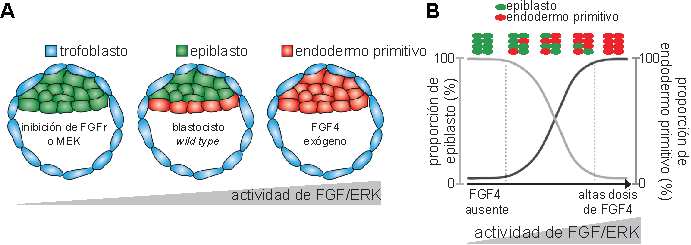
\includegraphics[width=1\columnwidth]{figures/chapter1/C1_saltandpepper.pdf} 
    \caption{\textbf{La señalización FGF4/ERK regula la composición del tejido interno del blastocisto.} (A) Representación de la composición del tejido interno del blastocisto cuando los niveles de actividad de la vía FGF/ERK son regulados experimentalmente. Figura adaptada de \cite{Brewer2016}. (B) Esquema del modelo de determinación estocástica dependiente de la señal FGF4/ERK de los linajes del tejido interno del blastocisto. El eje y indica la proporción de cada linaje. Figura adaptada de \cite{Yamanaka2010}. (A,B) El tejido interno del blastocisto está compuesto por células del epiblasto (verde) y del endodermo primitivo (rojo). El eje x indica el nivel de activación de la señal FGF/ERK.}
    \label{C1_fig:saltandpepper}
\end{figure}
%VER: no hice quilombo con FGF y FGF4?


%Luego de la implantación, las células del epiblasto evolucionan en el epiblasto postimplantatorio temprano. Con el correr de los días, las células del epiblasto postimplantatorio reciben un gran número de factores inductores provenientes del endodermo primitivo y el trofoblasto adyacentes . De esta manera, comienzan a especificarse dependiendo de su localización, generando un conjunto heterogéneo de células que eventualmente dará lugar a las tres capas germinales embrionarias y al endodermo extraembrionario \cite{Nakamura2016}.
% como factores de crecimiento fibroblásticos (FGFs)


\section{Células madre embrionarias como sistema modelo en biología del desarrollo}
\sectionmark{Células madre embrionarias}
\label{C1_sec:ESC}

Como condición general, las células madre se caracterizan por no estar al final de una vía de diferenciación, y tener la capacidad de dividirse sin límite, dando lugar a células hijas que pueden ser células madre- es decir, autorrenovarse- o células que emprendan el camino de la diferenciación celular. Hay muchos tipos de células madre, y las células madre embrionarias (ESCs, por \textit{embryonic stem cells}) son células derivadas de la masa celular interna del embrión de preimplantación (figura \ref{C1_fig:des_emb_temprano}) \cite{Ohtsuka2008}. Estas células se caracterizan por su gran potencial de diferenciación: si bien no pueden generar un organismo completo por sí mismas, son pluripotentes y tienen la capacidad de diferenciarse a todos los tipos celulares del individuo adulto, tanto \textit{in vitro} como en embriones quimeras -donde es posible integrarlas, y luego inyectar esos embriones en el útero materno de un organismo adulto para dar origen a ratones quimeras-\cite{Evans1981, Martin1981,Moustafa1972,Gardner1968}. Además, pueden ser mantenidas en cultivo, en teoría, indefinidamente \cite{Hiyama2007}. Por estas características, las células madre embrionarias son uno de los principales sistemas modelo para estudiar la diferenciación celular. 


Como mencionamos previamente, en el ratón la diferenciación de las células de la masa celular interna del embrión hacia el endodermo primitivo depende de la señalización de la vía FGF/RAS/RAF/MEK/ERK de manera dependiente de la dosis de FGF4 (figura \ref{C1_fig:saltandpepper}). En el embrión, FGF4 se expresa primero en las células de la masa celular interna, y luego se restringe a las células del epiblasto \cite{Guo2010}. Las células madre embrionarias son un sistema modelo manejable que recapitula esta función \cite{Raina2021,Schroeter2015,Kunath2007,Molotkov2017,Coumoul2003}. En este sistema, los ligandos FGF4 surgen de la señalización de las propias células madre. Tanto en el embrión como en las ESCs, los ligandos de FGF4 desencadenan la señalización de la proteína efectora ERK, y la señalización FGF/ERK regula la expresión de factores de transcripción \cite{Kang2013,Krawchuk2013,Kunath2007,Nichols2009,Boroviak2014,Stavridis2007}. 


%condiciones de cultivo que mantienen la pluripotencia de las ESCs 
Las células madre embrionarias de ratón (mESCs, por \textit{mouse embryonic stem cells}) pueden mantenerse en cultivo indefinidamente. Una forma de lograrlo es añadir al serum (o suero), que es un medio basal químicamente indefinido, la citoquina LIF (por \textit{leukemia inhibitory factor}). En estas condiciones de cultivo, el LIF junto con señales adicionales presentes en el serum promueve la autorrenovación de las ESCs, manteniéndolas indiferenciadas \cite{Smith1988,Ying2003,Ohtsuka2008,Morgani2013}. Es conocido que en este medio de cultivo, las mESCs presentan una elevada heterogeneidad poblacional, tanto en morfología como en la expresión de genes marcadores de pluripotencia. Esto sugiere que los cultivos de ESCs pueden albergar células con distinto potencial funcional \cite{Canham2010,Chambers2007,Hayashi2008,Kobashi2009,Singh2007,Toyooka2008,Yamanaka2010}. Además, al ser un medio químicamente indefinido, la vía de señalización de ERK es activada por el serum  y posiblemente haya otros factores que inhiban la diferenciación \cite{Roux2004,Lavoie2020}. En adelante, nos referiremos a este medio de cultivo como serum + LIF, o s+L.   


Las mESCs también pueden ser mantenidas en cultivo indiferenciadas en un medio mínimo químicamente definido. Por ejemplo, con los inhibidores PD0325901 (en adelante, MEKi por \textit{MEK inhibitor}), un inhibidor de la proteína MEK que activa a ERK, y CHIR99021 (en adelante, chiron), un inhibidor de la proteína GSK3 (por \textit{glycogen synthase kinase 3}) \cite{Marks2012}. Estos dos inhibidores -a los que comúnmente se los conoce como ‘2i’- protegen a las ESCs de las señales inductoras de diferenciación, y los cultivos presentan una mayor homogeneidad poblacional en morfología y en la expresión de genes marcadores de pluripotencia \cite{Nichols2009,Wray2010,Wray2011}. En esta formulación 2i, inhibir la señalización de ERK mediante su activador MEK es esencial para la autorrenovación de ESCs de ratón, pues se impide la diferenciación impulsada por ERK \cite{Lavoie2020,Chen2015,Lavoie2020,Weinberger2016}. El cultivo 2i a menudo se complementa con LIF para tener cultivos más homogéneos, y se suele usar N2B27 (serum free) como medio basal \cite{Morgani2013,Ying2008}. Se ha demostrado que las células madre embrionarias pueden ser mantenidas en cultivo indiferenciadas con sólo dos de los tres componentes del medio 2i+LIF. 

%Sin embargo, la ablación genética de ERK es perjudicial para mantener la supervivencia de la célula y produce un fenotipo diferente al que se obtiene inhibiendo MEK. Esto sugiere que la inhibición de MEK tiene funciones adicionales en el mantenimiento de la estabilidad de las ESCs que son independientes de la ablación de ERK \cite{Chen2015,Lavoie2020,Weinberger2016}

% cell cycle
Para finalizar, durante el desarrollo embrionario temprano, las células del embrión cercano a la implantación tienen la capacidad de proliferar a un ritmo inusualmente rápido y generan, así, la expansión del volumen embrionario. Este fenómeno se recapitula en las mESCs cultivadas \textit{in vitro} en serum+LIF y en 2i+LIF, donde presentan una duración del ciclo celular de entre 11 y 14 horas \cite{Waisman2019,Snow1977}. Estos tiempos son sorprendentemente rápidos en comparación con las 24 horas que suele durar el ciclo celular en algunas células diferenciadas de manera terminal. 



\section{Diferenciación de células madre embrionarias en células madre epiblasto}
\sectionmark{Células madre epiblasto}
\label{C1_sec:EpiSCs}
%EpiSCs 
Cuando las ESCs están en cultivo y se remueven los factores que mantienen la pluripotencia, se diferencian como si continuaran con el desarrollo embrionario \cite{Keller1995,Keller2005}. Se observó que las mESCs pueden diferenciarse a células madre epiblasto (EpiSCs, por \textit{epiblast stem cells}), células similares a las del epiblasto (figura \ref{C1_fig:des_emb_temprano}) \cite{Kojima2014,Brons2007}. Estas células, que también pueden obtenerse directamente desde embriones, son células madre pluripotentes que tienen la capacidad de dar lugar a todas las células del organismo maduro, pero se encuentran en un estadío de diferenciación posterior a las ESCs. Al igual que las mESCs, las mEpiSCs expresan marcadores de pluripotencia, pero tienen patrones de expresión génica y respuestas de señalización distintas a las de mESCs, que normalmente funcionan en el epiblasto \cite{Tesar2007}. También, a diferencia de las mESCs, las mEpiSCs son ineficientes para colonizar de forma funcional luego de inyectarlas en un blastocisto.

%Las EpiSCs parecen estar en estados heterogéneos, y expresan marcadores asociados a distintas capas germinales, lo que probablemente refleje su origen de una población celular heterogénea en el epiblasto postimplantatorio. 

%Las mESCs son conducidas a la diferenciación en EpiSCs por la señalización FGF/ERK \cite{Kunath2007,Stavridis2007}, y las señales que controlan su diferenciación son distintas a las de las ESCs.


Las mEpiSCs requieren de la señalización de Activina (Nodal) y factores de crecimiento de fibroblastos (FGFs, por \textit{fibroblast grow fators}) para mantener sus cultivos indiferenciados. Además, se ha observado la señalización canónica de Wnt impide la autorrenovación de las EpiSCs y promueve su diferenciación hacia una de las capas germinales. El inhibidor XAV939 para bloquea esta diferenciación espontánea y potencia la expresión de genes indicadores de pluripotencia, permitiendo la propagación de las EpiSCs como una población homogénea \cite{Guo2009,Tsukiyama2014,Brons2007,Sumi2013,Ying2003,Weinberger2016}. 


En este trabajo utilizaremos a las EpiSCs como ejemplo de células levemente más diferenciadas que las ESCs. El medio de cultivo que emplearemos es N2B27 como medio basal, suplementado con FGF2, activina y XAV939, que comúnmente se lo conoce como FAX \cite{Brons2007}.
%Sin embargo, la diferenciación de CMEr a EpiSCs conlleva alrededor de 5-7 días en cultivo



\section{Sistema de señalización FGF/ERK en células madre embrionarias}
\sectionmark{Sistema de señalización FGF/ERK}
\label{C1_sec:FGF_ERK}

%cite Dessauges

 %chequear estas citas!
La vía de señalización FGF/ERK tiene funciones críticas y generalizadas durante el desarrollo embrionario temprano \cite{Kang2013,Nichols2009,Yamanaka2010,Krawchuk2013,Kang2017,Molotkov2017,Nichols2009,Morgani2013}. Entre muchas otras funciones, es necesaria para generar y/o mantener los tres linajes del embrión de preimplantación: el epiblasto, el endodermo primitivo y el trofoblasto (figura \ref{C1_fig:des_emb_temprano}). En particular, regula la especificación de células de la masa celular interna en el endodermo primitivo (figura \ref{C1_fig:saltandpepper}). Además, también está involucrado en la maduración de las células pluripotentes del epiblasto, y FGF es esencial para el aislamiento y mantenimiento de las EpiSCs \cite{Brons2007,Tesar2007}. 


Los factores de crecimiento de fibroblastos (FGFs) son una familia de proteínas de señalización. Una amplia gama de genes \textit{Fgf} se han identificado en vertebrados, siendo 22 en ratones y humanos \cite{Thisse2005}. La expansión de las familias de genes \textit{Fgf} y \textit{Fgfr} a lo largo de la evolución de organismos multicelulares ha permitido que este sistema de señalización adquiera diversidad funcional y, por tanto, una participación casi ubicua en procesos fisiológicos y de desarrollo \cite{Itoh2004,Powers2000,Goldfarb1996,Coumoul2003}. 


%esto es general de todos los receptores de FGF?
18 de las 22 proteínas FGF identificadas se unen y activan los 4 receptores de tirosina quinasa FGFr. Estos receptores son monómeros inactivos \cite{Schlessinger2000}. Su dimerización, o activación, promueve la autofosforilación de residuos de tirosina intracelulares específicos, y esta activación representa el primer paso para iniciar la cascada de señalización de los receptores FGFr. Entonces, la interacción de los ligandos FGF con sus receptores resulta en la activación de una serie de vías de señalización, y en mESCs la principal es la vía de quinasas activada por mitógenos RAS/RAF/MEK/ERK (figura \ref{C1_fig:FGF_ERK_pathway}). Cuando se activa la vía de señalización, proteínas de señalización intracelular transmiten la señal dentro de la célula. Esta transmisión la realizan regulando la activación de otras proteínas de señalización río abajo de la red, por ejemplo a través de reacciones de fosforilación y desfosforilación \cite{Johnson1996}. 


 \begin{figure}
    \centering
    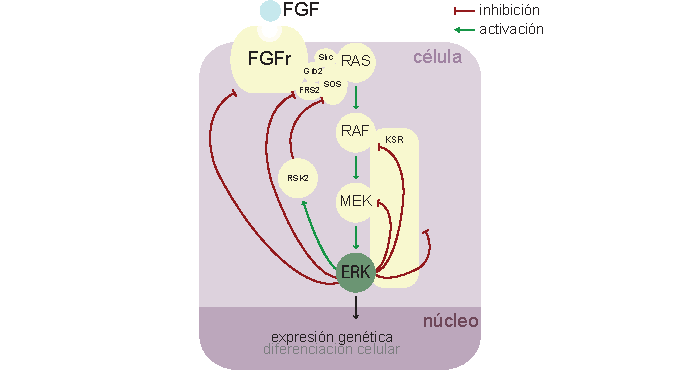
\includegraphics[width=1\columnwidth]{figures/chapter1/C1_FGF-ERK_pathway.pdf} 
    \caption{\textbf{Esquema del sistema de señalización celular FGF/ERK.} Para simplificar, sólo se incluyen algunos bucles de retroalimentación como ejemplo. Figura basada en \cite{Lake2016}.}
    \label{C1_fig:FGF_ERK_pathway}
\end{figure}

En particular, las quinasas son enzimas capaces de fosforilar, y así regular la actividad, de proteínas intracelulares. Estas enzimas contienen sitios activos que reconocen una secuencia de aminoácidos alrededor del sitio de fosforilación \textit{target} en la proteína blanco correcta, y a menudo contienen sitios de acoplamiento adicionales que promueven una interacción específica y de alta afinidad con el objetivo. Muchas proteínas de señalización intracelular controladas por la fosforilación son también quinasas que a menudo se organizan en cascadas, como la vía de quinasas activada por mitógenos RAS/RAF/MEK/ERK. En estas cascadas, una quinasa que se activa por fosforilación, fosforila una o más proteínas quinasas río abajo de la red, y así sucesivamente, transmitiendo y amplificando la señal, o extendiéndola a otras vías de señalización. La fosforilación es un proceso reversible, de modo que las reacciones pueden activarse o desactivarse en respuesta a diferentes estímulos  \cite{Rosen1983,Pawson2005}. Las fosfatasas catalizan la desfosforilación y son reguladores negativos clave en los sistemas de señalización celular \cite{Lemmon2016}.  


En concreto, FGFr activo promueve la fosforilación de la proteína adaptadora FRS2$\alpha$, reclutada para completar la activación del receptor y permitir la unión de la pequeñas moléculas adaptadoras (figura \ref{C1_fig:FGF_ERK_pathway}). Luego, la autofosforilación de los residuos de el receptor FGFr actúa como sitio de reconocimiento de las proteínas adaptadoras Shc y Grb2, entre otras. Estas proteínas reclutan a SOS desde el citosol hacia la membrana plasmática, quien participa en la activación de la proteína de unión GDP-RAS. En este complejo, SOS cataliza el intercambio de GDP por GTP, promoviendo la activación de RAS \cite{Lake2016,Thisse2005,Alberts2008,Lavoie2020}. La activación de RAS recluta a RAF hacia la membrana plasmática, donde se activa y conduce a la activación de la cascada de proteínas que pertenecen a la familia de quinasas activadas por mitógenos (MAPKs, por \textit{mitogen activated protein kinases}). 


Los tres componentes de esta familia forman un módulo de señalización funcional que se ha conservado notablemente durante la evolución y se utiliza, con variaciones, en muchos contextos de señalización diferentes. Estos componentes son proteínas quinasas \cite{Roux2004}. La última quinasa de la serie es la MAP quinasa (MAPK, por \textit{mitogen activated protein kinase}). La siguiente en la serie es la MAP quinasa quinasa (MAPKK), que fosforila y activa la MAP quinasa. Por último, la que recibe una señal de activación directamente de RAS es la MAP quinasa quinasa (MAPKKK), que fosforila y activa la MAPKK. En mamíferos, la MAPKKK se conoce como RAF (por \textit{rapidily accelerated fibrosarcoma}), la MAPKK como MEK (por \textit{mitogen activated ERK kinase}), y la MAPK como ERK\footnote{A menos que se especifique lo contrario, utilizaremos el término ``ERK''  para referirnos a las proteínas ERK1 y ERK2. Aplicamos la misma simplificación a otras proteínas que tienen múltiples isoformas, como por ejemplo FGFr, RAS, RAF, RSK, MEK.}(por \textit{extracellular signal regulated kinase}) (figura \ref{C1_fig:FGF_ERK_pathway}). Finalmente, ERK activa, o fosforilada, funciona como proteína efectora. Se reubica en varios compartimentos subcelulares y modula por fosforilación la actividad de un amplio conjunto de sustratos, incluyendo la capacidad de promover la transcripción de determinados factores dentro del núcleo, lo que conduce a respuestas específicas de la célula según su origen y estado de desarrollo (figura \ref{C1_fig:FGF_ERK_pathway}).


Para adaptarse a determinadas circunstancias ambientales, la vía RAS/RAF/MEK/ERK debe integrarse en la actividad de señalización global de la célula. La regulación de esta vía de señalización es compleja e incluye numerosos bucles de retroalimentación positiva y negativa, que probablemente evolucionaron para conferir un control eficaz de esta vía de señalización evolutivamente conservada \cite{Lake2016,Dougherty2005,Ekerot2008,Lavoie2015,Lemmon2016,Nett2018,Sturm2010}. Esos bucles pueden combinarse de distintas formas, y son los responsables de dar como respuesta distintos patrones dinámicos de la actividad de ERK. Algunos bucles conocidos de esta red de señalización se encuentran representados en la figura \ref{C1_fig:FGF_ERK_pathway}. En la próxima sección presentamos algunos ejemplos de posibles patrones dinámicos de la actividad de ERK que se han observado previamente. 


%Aunque es esencial para el funcionamiento normal de la célula, su capacidad de "recablear" las vías de señalización representa un gran problema para la innovación clínica. En las últimas décadas se ha avanzado mucho en la comprensión de la compleja regulación de la señalización señalización ERK1/2 MAPK. Aunque todavía hay un gran número de de preguntas abiertas, estamos empezando a ver los beneficios de de la aplicación de estos conocimientos al tratamiento del cáncer en la clínica.



\section{Respuesta dinámica de ERK en diferentes contextos}
\label{C1_sec:ERK}

Como condición general, estudiar la dinámica de una proteína efectora- es decir, su actividad en función del tiempo- cuya actividad surge de una red intracelular de transducción de señales requiere realizar mediciones de la actividad de esta proteína en células únicas y vivas. La actividad de ERK en células únicas y vivas puede monitorearse con biosensores basados en el principio de transferencia de energía por resonancia de Förster o fluorescencia (FRET, por \textit{fluorescence resonance energy transfer}) \cite{Komatsu2011}. En el FRET, se transfiere energía entre dos fluoróforos, donante y aceptor, cuyos espectros de emisión (donante) y de excitación (aceptor) son compatibles. Entonces, si el donante es excitado, puede transferir energía al aceptor, que en ese caso emite fluorescencia. Esta transmisión de energía se produce si la distancia entre ellos es lo suficientemente corta, y su orientación relativa la apropiada, entre otros factores. Entonces, los biosensores FRET unimoleculares contienen proteínas fluorescentes donantes y aceptoras  \cite{JaresErijman2003,Miyawaki2003}. Para medir la actividad de ERK en células únicas y vivas, se integra a las células un sensor diseñado para que la quinasa ERK en su estado activo, fosforile el sustrato del sensor. Esta fosforilación conduce a un cambio en la conformación del sensor FRET, que promueve la transferencia de energía entre el donante y el aceptor. Luego, excitando al donante, los niveles de intensidad de fluorescencia que se adquieren en el rango de emisión del aceptor se corresponden con mayores niveles de actividad de ERK. Se suele cuantificar esta medición mediante el cociente entre la adquisición en el canal del aceptor y el donante, magnitud que se suele denominar cociente FRET. También se puede realizar mediciones de la actividad de ERK con otro tipo de sensores cuya lectura es su localización dentro de la célula. Por ejemplo, es posible construir un sensor cuya fosforilación, mediada por ERK activa, desplace al sensor acoplado a una proteína fluorescente desde el núcleo hacia el citoplasma \cite{Regot2014}. En este tipo de sensores, comúnmente llamados de traslocación, el cociente de fluorescencia citoplasmática/nuclear puede ser interpretado como un \textit{proxy} de la actividad de ERK.


%CITE \cite{Hamilton2019}
Trabajos previos estudiaron la actividad de ERK en ESCs que expresan un sensor basado en FRET estimuladas de forma aguda, es decir, se realizaron mediciones de la actividad de ERK inmediatamente después de remover un inhibidor de su proteína activadora MEK. Este análisis reveló un pico transitorio de actividad cuyo máximo aparecía aproximadamente 40 minutos luego de la remoción del inhibidor, y decaía gradualmente en escalas de tiempo largas, del orden de varias horas \cite{Deathridge2019}. También observaron que este decaimiento era heterogéneo a lo largo de la población celular. 

Que el estímulo y las mediciones realizadas comiencen en el mismo momento nos aporta información sobre la respuesta transitoria de la activación de ERK. Sin embargo, también es razonable realizar mediciones una vez que se haya alcanzado el estado estacionario, pues modela con mayor precisión la respuesta celular a la exposición crónica del ligando, necesarios para desencadenar la diferenciación de las ESCs y como se cree que ocurre en el desarrollo embrionario. En particular, la dinámica de señalización de ERK en escalas temporales cortas en los regímenes de estimulación continua de FGF no están explorados hasta el momento. 
%La dinámica de ERK a corto plazo nos otorgaría información sobre la arquitectura de la red que la regula, así como también es importante en la expresión de algunos genes de genes tempranos que pueden ser factores de transcripción. 


La dinámica de activación de ERK en escalas temporales cortas y con estimulación continua del receptor del factor de crecimiento epidérmico (EGF, por \textit{epidermal grow factor}) - un receptor de tirosina quinasa que regula la actividad de ERK en muchas células más diferenciadas que las ESCs- se estudió en otros tipos celulares y muestra comportamientos muy diversos. En muchos tipos celulares, pero no en todos, se reportó que la actividad de ERK era pulsátil, y que dicha actividad pulsátil era estocástica \cite{Aoki2013}. En otros tipos celulares, se reportó que la actividad de ERK era oscilatoria \cite{Shankaran2009}, o simplemente se observaron pulsos discretos \cite{Albeck2013}.


%En varios casos, la frecuencia de los pulsos de actividad ERK depende de la concentración de EGF o de la densidad celular \cite{Albeck2013,Aoki2013}. Esto ha llevado a sugerir que la red RAS/RAF/MEK/ERK, cuya actividad es desencadenada por la activación del receptor de EGF, codifica la información sobre los niveles de la señal extracelular con una frecuencia modulada \cite{Albeck2013}. En cambio, en otros tipos celulares, los pulsos de translocación nuclear de ERK tienen una frecuencia constante en un rango de niveles de estimulación de EGF \cite{Shankaran2009}. 



\section{Objetivos, esquema de trabajo y posibles aplicaciones}


Como resumen, la diferenciación de las células del embrión de preimplantación de ratón en el tipo celular endodermo primitivo depende de la red de señalización FGF/ERK, principalmente estimulada por la señalización de FGF4 que produce el mismo tejido. Las células madre embrionarias son un sistema modelo manejable que recapitula estas características. Se ha mostrado que la señalización de ERK es altamente dinámica en otros contextos biológicos. A pesar de que las funciones de FGF/ERK durante la diferenciación en ESCs son conocidas, su dinámica de señalización en este contexto de desarrollo está poco estudiada. En particular, la dinámica de señalización de ERK en escalas temporales cortas está hasta el momento inexplorada.


Con un enfoque interdisciplinario, en esta tesis nos preguntamos, a nivel celular, (i) cómo es la dinámica de activación de ERK en células madre embrionarias de ratón; (ii) cuáles de sus rasgos dinámicos constituyen información sobre los estímulos extracelulares y las características, tanto definitorias como transitorias, del tipo celular. Además, a nivel poblacional, (iii) qué tan homogénea es la respuesta de activación de ERK en una población de células en estos distintos contextos.


Para responder estas preguntas, primero empleamos y desarrollamos métodos de análisis para obtener información cuantitativa de mediciones de la actividad dinámica de ERK en distintos contextos y escalas temporales. Esta descripción cuantitativa será fundamental para construir una descripción conceptual de la dinámica de activación de ERK en células madre embrionarias. Luego nos proponemos resumir en una descripción teórica de baja dimensionalidad las ideas más importantes que surjan de este análisis, buscando describir y comprender la dinámica de activación de ERK en ESCs.


Las células madre embrionarias no solo constituyen un sistema experimental interesante para estudiar el desarrollo embrionario, sino que también son una importante promesa para distintas áreas de la medicina \cite{Garreta2021,Waisman2019}. En este marco, realizar una descripción cuantitativa y teórica de la dinámica de señalización celular de la vía FGF/ERK busca ser un aporte para revelar los mecanismos de regulación de la red de señalización y/o predecir las respuestas celulares, conocimientos fundamentales para el desarrollo de estas áreas \cite{Shankaran2009}. Por ejemplo, la comprensión los mecanismos que gobiernan los procesos de diferenciación celular es crucial para desarrollar técnicas de diferenciación celular dirigida, técnicas sumamente útiles en el desarrollo de la medicina regenerativa, en la investigación de enfermedades o en el monitoreo y testeo de drogas experimentales \cite{Keller2005,Inoue2014}. Por otro lado, estos conocimientos son relevantes para desarrollar nuevos tratamientos en los casos en que falla la elección del destino celular. Debido a su papel central en las decisiones de destino celular, la desregulación de la red de ERK conduce a varias enfermedades, como por ejemplo el cáncer \cite{Dessauges2022,Bugaj2018,Lavoie2020,Grieco2013}, y los resultados de esta tesis podrían ser relevantes para desarrollar tratamientos contra esas enfermedades. Como complemento, esperamos poder aportar nuevos conocimientos en el área de procesos estocásticos y dinámica no lineal, motivados por nuevas preguntas que surjan de la caracterización cuantitativa del sistema biológico que estudiamos y queremos describir.

 

Comenzamos esta tesis enfocándonos en una de las partes más básicas e importantes de este trabajo. En el capítulo \ref{ch2} nos preguntamos cómo es la dinámica de activación de ERK en células madre embrionarias de ratón en condiciones de cultivo que mantienen la pluripotencia. Utilizamos un sensor cuya lectura es su localización dentro de la célula para medir la dinámica de la actividad de la ERK en ESCs vivas e individuales, enfocándonos en escalas temporales cortas. Para analizar las series temporales de actividad de ERK que surgen de los experimentos, desarrollamos un protocolo de análisis de señales para caracterizar sus principales rasgos dinámicos, protocolo que utilizaremos en el resto del trabajo. Luego, definimos métricas que nos permiten comparar las observaciones experimentales con modelos teóricos simples previamente sugeridos por la bibliografía. A partir de estas observaciones, en el capítulo \ref{ch3} nos preguntamos cómo cambian las principales propiedades de la dinámica de activación de ERK ante perturbaciones experimentales. Primero, cómo se modifica la dinámica de activación de ERK en ESCs ante exponer a la célula a distintas concentraciones controladas de ligando FGF4. Luego, qué aspectos de la dinámica de ERK son propios de este estadío de diferenciación, y comparamos la dinámica de activación de ERK en ESCs y células madre epiblasto. Prosiguiendo, en el capítulo \ref{ch4} estudiamos posibles variaciones de escalas temporales largas de la dinámica de actividad de ERK en células individuales, comparables con el ciclo celular. Desarrollamos nuevos protocolos experimentales que nos permiten adquirir la señal de actividad de ERK durante todo el ciclo celular. Estas nuevas series temporales son más largas, pero de menor resolución, e implementamos una nueva estrategia de análisis que nos permiten estudiar posibles variaciones de la actividad de ERK a lo largo del ciclo celular. Como continuación, buscamos resumir las ideas surgidas en los capítulos anteriores en un modelo matemático de baja dimensionalidad, es decir, pocas variables. Comenzamos por un modelo simple y conocido, que iremos modificando a partir del diálogo entre la teoría y los experimentos que realizamos previamente. Con este enfoque, a modo casi introductorio, en el capítulo \ref{ch5} presentamos la dinámica de un modelo de fase con bifurcación de ciclo infinito. Este modelo, de naturaleza determinista, no es a simple vista suficiente para describir nuestras observaciones. Extendemos nuestra propuesta a una descripción de naturaleza estocástica, y estudiamos un modelo de fase con bifurcación de ciclo infinito con ruido blanco gaussiano aditivo. Este modelo es el punto de partida para establecer el diálogo entre experimentos y teoría, y en el capítulo \ref{ch7} desarrollamos un procedimiento que permite ajustar y comparar el modelo propuesto con los experimentos. A partir de los resultados del ajuste, proponemos modificaciones al modelo del capítulo anterior, que ajustamos y comparamos con nuestros resultados experimentales. Para terminar, en el capítulo \ref{ch8} discutimos nuestros resultados y formulamos nuevas preguntas que surgen de ellos.

\end{document}